\documentclass[12pt]{report}

% Page layout
\usepackage[a4paper, margin=1in]{geometry}

% Mathematics
\usepackage{amsmath, amssymb}

% Encoding
\usepackage[utf8]{inputenc}

% Figures and tables
\usepackage{graphicx}
\usepackage{float}

% Formatting
\usepackage{setspace}
\usepackage{titlesec}
\usepackage{tocbibind}

% URLs and colors
\usepackage{url}
\usepackage{xcolor}

% Code listings
\usepackage{listings}

\lstset{
    language=Python,
    basicstyle=\ttfamily\footnotesize,
    keywordstyle=\bfseries,
    commentstyle=\itshape,
    stringstyle=\ttfamily,
    showstringspaces=false,
    breaklines=true,
    breakatwhitespace=true,
    frame=single,
    numbers=left,
    numberstyle=\tiny,
    tabsize=4,
    captionpos=b
}

% Chapter title format
\titleformat{\chapter}[hang]
  {\normalfont\huge\bfseries}
  {\thechapter.}
  {1em}
  {}

% Thesis title information
\title{Numerical Methods for Solving Nonlinear Equations and Systems of Nonlinear Equations}
\author{
Serhet G\"okdemir \\
21058024 \\[1em]
Advisor: Prof. Dr. Hale Gonce K\"o\c{c}ken
}
\date{Istanbul, 2026}

\begin{document}

\maketitle

\clearpage
\pagenumbering{roman}

% Front matter
\begin{flushleft}
\textcopyright\ All rights of this thesis belong to Yıldız Technical University, Department of\\
Mathematical Engineering.
\end{flushleft}
\chapter*{Abstract}
\addcontentsline{toc}{chapter}{Abstract}

This thesis investigates numerical methods for solving nonlinear equations and systems of nonlinear equations. Such problems arise frequently in various areas of science, engineering, optimization, and computational mathematics, and in many practical cases their exact analytical solutions cannot be obtained. For this reason, numerical approaches play an important role in approximating their solutions.

The study focuses on both single nonlinear equations and systems of nonlinear equations. For single-variable problems, the bisection method, secant method, Newton's method, damped Newton method, and Brent's method are examined. For nonlinear systems, multivariable Newton and Broyden methods are studied. The theoretical foundations, convergence properties, advantages, limitations, and failure cases of these methods are discussed.

In addition to the theoretical analysis, the selected numerical methods are implemented in Python using a modular computational structure. Numerical experiments are performed in order to compare the methods in terms of convergence behavior, residual reduction, and stability. Convergence plots, residual analyses, and iteration histories are used to evaluate the performance of the algorithms.

The thesis also investigates the relationship between nonlinear equation solving and optimization techniques. In particular, residual minimization, Newton-type optimization methods, damping strategies, line-search techniques, and the Armijo condition are discussed from an optimization perspective. An adaptive damped Newton method based on Armijo backtracking is also implemented and analyzed numerically.

Overall, the study combines theoretical numerical analysis with practical computational implementation and provides a structured examination of numerical methods for nonlinear problems.
\chapter*{Preface}
This thesis has been prepared as part of the undergraduate studies in Mathematical Engineering at Yıldız Technical University.

The main motivation behind this work is the author’s interest in numerical methods and optimization techniques. During the study, an effort has been made to understand the fundamental principles of solving nonlinear equations and to explore their practical implementations.

The author would like to express sincere gratitude to the advisor, Prof. Dr. Hale Gonce Köçken, for her guidance, support, and valuable insights throughout the preparation of this thesis.
\addcontentsline{toc}{chapter}{Preface}
\vspace{1cm}
\chapter*{Symbols}
\addcontentsline{toc}{chapter}{Symbols}

\begin{tabular}{ll}
\(f(x)\) & Scalar nonlinear function \\[0.3cm]
\(F(\mathbf{x})\) & Vector-valued nonlinear function \\[0.3cm]
\(x^*\) & Exact root or solution \\[0.3cm]
\(x_k\) & Approximation at iteration \(k\) \\[0.3cm]
\(\mathbf{x}_k\) & Vector approximation at iteration \(k\) \\[0.3cm]
\(e_k\) & Error at iteration \(k\) \\[0.3cm]
\(J_F(\mathbf{x})\) & Jacobian matrix of \(F\) \\[0.3cm]
\(\mathbf{s}_k\) & Iteration step vector \\[0.3cm]
\(\alpha_k\) & Damping or step-size parameter \\[0.3cm]
\(\varepsilon\) & Tolerance parameter \\[0.3cm]
\(\|\mathbf{x}\|\) & Euclidean norm of vector \(\mathbf{x}\) \\[0.3cm]
\(B_k\) & Approximate Jacobian matrix in Broyden's method \\[0.3cm]
\(p\) & Order of convergence \\[0.3cm]
\(C\) & Constant used in convergence analysis \\[0.3cm]
\(\mathbf{0}\) & Zero vector \\[0.3cm]
\(\mathbb{R}^n\) & \(n\)-dimensional real vector space \\[0.3cm]
\(\phi(\mathbf{x})\) & Merit or residual objective function \\[0.3cm]
\(\Delta_k\) & Trust-region radius \\[0.3cm]
\(g(x)\) & Fixed-point iteration function \\[0.3cm]
\(L\) & Contraction constant \\[0.3cm]
\(\rho\) & Backtracking reduction factor \\[0.3cm]
\(c\) & Armijo sufficient decrease parameter \\[0.3cm]
\end{tabular}
\vspace{1cm}
\chapter*{Abbreviations}
\addcontentsline{toc}{chapter}{Abbreviations}

\begin{tabular}{ll}
NumPy & Numerical Python Library \\[0.3cm]
Pandas & Python Data Analysis Library \\[0.3cm]
Jupyter & Interactive computational notebook environment \\[0.3cm]
\end{tabular}

\vspace{1cm}

\tableofcontents
\listoffigures
\listoftables

\clearpage
\pagenumbering{arabic}

% Chapters
\chapter{\MakeUppercase{Introduction}}

\section{Motivation Behind Numerical Methods}

There are two basic approaches one may apply while trying to solve any mathematical problem: solving analytically or numerically. The process of solving analytically refers to calculating the exact solution of the given problem. It is possible to calculate the solution of many classical mathematical problems analytically and thus to derive the exact solution.

Nevertheless, there are many problems for which the analytical solution either does not exist at all or its calculation is excessively expensive. For instance, nonlinear and systems of nonlinear equations often cannot be solved analytically; thus, other methods have to be used.

Unlike the analytic approach, numeric methods allow deriving an approximate solution with a required precision. These methods utilize iterative algorithms that make it possible to gradually improve an approximation up until the required precision is obtained.

Different numerical methods have their own advantages and disadvantages. These advantages and disadvantages can be their convergence rates, computational costs and stability. So, selecting an appropriate method for a given problem has an important role. \cite{burden, atkinson}.

\section{Nonlinear Equations and Systems}

A nonlinear equation is an equation of the form
\begin{equation}
f(x) = 0,
\end{equation}
\noindent where \( f \) is a nonlinear function. In contrast to linear equations, nonlinear equations may exhibit multiple roots, no real roots, or complex solution structures, making their analysis and solution more challenging \cite{burden, atkinson}.

A simple example of a nonlinear equation is

\begin{equation}
f(x) = x^3 - x - 2 = 0
\end{equation}

for which no closed-form analytical solution exists in a simple form. Such equations commonly arise in various scientific and engineering applications, including physics, optimization, and computational modeling.

However, in practice, there exist cases where obtaining an exact analytical solution for a nonlinear equation is not feasible. If at all an analytical solution is obtainable, it might prove to be extremely complex to compute. This is why numerical solutions are sought after in order to obtain the roots of the nonlinear equation.

The problem can be extended to systems of nonlinear equations. 
A nonlinear system can be written in vector form as
\begin{equation}
F(\mathbf{x}) = \mathbf{0},
\end{equation}
where
\begin{equation}
F : \mathbb{R}^n \to \mathbb{R}^n
\end{equation}
is a vector-valued nonlinear function.

For example, consider the system
\begin{equation}
\begin{cases}
x^2 + y^2 - 4 = 0, \\
x - y - 1 = 0.
\end{cases}
\end{equation}

\noindent Such systems arise naturally in applications where multiple variables interact in a nonlinear manner.

Solving a nonlinear system is usually more complex than solving a single nonlinear equation. Moreover, solution methods often require use of Jacobian matrix. It is defined as

\begin{equation}
J_F(\mathbf{x}) =
\begin{bmatrix}
\frac{\partial f_1}{\partial x_1} & \frac{\partial f_1}{\partial x_2} & \cdots & \frac{\partial f_1}{\partial x_n} \\
\frac{\partial f_2}{\partial x_1} & \frac{\partial f_2}{\partial x_2} & \cdots & \frac{\partial f_2}{\partial x_n} \\
\vdots & \vdots & \ddots & \vdots \\
\frac{\partial f_n}{\partial x_1} & \frac{\partial f_n}{\partial x_2} & \cdots & \frac{\partial f_n}{\partial x_n}
\end{bmatrix}.
\end{equation}

which generalizes the concept of the derivative to higher dimensions \cite{kelley}.
In this thesis, both one-dimensional and multidimensional nonlinear equations will be studied. It will be particularly focused on the iterative techniques used to solve these equations numerically, taking into consideration issues such as convergence and cost.

\section{Objectives of the Thesis}

The primary aim of this dissertation is the analysis of numerical methods used in finding solutions of nonlinear equations and nonlinear equation systems. This kind of problem often occurs in different branches of science and technology; in many cases, there are no analytical solutions to such problems. For this reason, numerical methods take the lead in solving them. \cite{burden, atkinson}.

In this context, the thesis focuses on two main classes of problems. The first involves numerical methods for solving single nonlinear equations of the form \( f(x) = 0 \). Classical approaches, including the bisection, secant, and Newton-type methods, are examined with emphasis on their basic principles and convergence characteristics.

The second part of the study considers systems of nonlinear equations of the form \( F(\mathbf{x}) = \mathbf{0} \). Compared with single equations, these systems are generally more complex and often require more advanced solution techniques, especially those based on the Jacobian matrix. The methods used to solve such systems are investigated within a similar theoretical framework.

In addition to the theoretical analysis, the selected numerical methods are implemented in Python using a consistent computational structure. The implementations are used to investigate the practical behavior of the methods through numerical experiments. In particular, the methods are compared in terms of convergence behavior, residual reduction, and robustness.

Overall, the aim of this thesis is to provide a clear and structured examination of numerical methods for nonlinear problems, combining theoretical foundations with computational analysis.

\section{Structure of the Thesis}

This thesis is divided into eight chapters.

Chapter 1 explains the motivation for studying numerical methods and introduces the concepts of nonlinear equations and systems of nonlinear equations. The aims of the thesis and the topics covered throughout the study are also outlined.

Chapter 2 provides the mathematical background needed for the methods discussed in the following chapters. Concepts such as fixed-point formulations, convergence analysis, orders of convergence, norms, Jacobian matrices, and stopping criteria are presented as the foundation for the later discussions.

Chapter 3 deals with numerical methods for solving single nonlinear equations. Well-known methods, including the bisection method, secant method, Newton’s method, damped Newton method, and Brent’s method, are introduced and discussed in terms of their convergence behavior. The chapter also includes illustrative examples and examples of situations in which these methods may fail.

Chapter 4 turns to systems of nonlinear equations. Multivariable Newton’s method and Broyden’s method are examined from both theoretical and computational perspectives. Several examples are provided to illustrate their application and to compare their convergence performance.

Chapter 5 focuses on the practical implementation of the numerical methods considered in the thesis. The structure of the repository, the Python implementations, the testing procedures, and issues related to reproducibility are discussed.

Chapter 6 presents the numerical experiments and comparative analyses carried out in this study. Benchmark problems, convergence plots, residual analyses, and experimental results are reported for both single-variable equations and systems of nonlinear equations, allowing the performance of the methods to be evaluated under different conditions.

Chapter 7 explores the connection between nonlinear equation solving and optimization. Topics such as residual minimization, Newton-type optimization methods, damping strategies, line-search techniques, and the Armijo condition are discussed from an optimization viewpoint. The chapter also includes a numerical investigation of an adaptive damped Newton method that employs Armijo backtracking.

Chapter 8 concludes the thesis by summarizing the main results obtained. The limitations of the work are discussed and several possible directions for future research are suggested.
\input{chapters/02-mathematical_background}
\chapter{\MakeUppercase{Single Nonlinear Equations}}

\section{Bisection Method}

The bisection method is one of the simplest and most reliable numerical techniques for solving nonlinear equations of the form \( f(x) = 0 \). It is based on the Intermediate Value Theorem, which states that if a continuous function \( f \) changes sign over an interval \([a, b]\), then there exists at least one root in that interval \cite{burden, atkinson}.

More precisely, if
\begin{equation}
f(a) \cdot f(b) < 0,
\end{equation}
then there exists a point \( c \in (a, b) \) such that
\begin{equation}
f(c) = 0.
\end{equation}

The method starts with such an interval \([a, b]\) and repeatedly bisects it. At each iteration, the midpoint is computed as
\begin{equation}
c_k = \frac{a_k + b_k}{2}.
\end{equation}

The value of the function at the midpoint, \( f(c_k) \), is then evaluated. Depending on the sign of \( f(c_k) \), the interval is updated as follows:

\begin{itemize}
    \item If \( f(a_k) \cdot f(c_k) < 0 \), then the root lies in \([a_k, c_k]\), so set \( b_{k+1} = c_k \).
    \item Otherwise, the root lies in \([c_k, b_k]\), so set \( a_{k+1} = c_k \).
\end{itemize}

This process is repeated until a stopping criterion is satisfied, such as the interval length becoming sufficiently small or the function value approaching zero.

One of the main advantages of the bisection method is its guaranteed convergence. As long as the function is continuous and the initial interval satisfies the sign change condition, the method will always converge to a root \cite{burden}.

However, the method has a relatively slow rate of convergence. The error decreases linearly, and the interval length is halved at each iteration. More precisely, after \( k \) iterations, the error satisfies

\begin{equation}
|x_k - x^*| \leq \frac{b_0 - a_0}{2^k}.
\end{equation}

This linear convergence makes the method less efficient compared to methods such as Newton's method or the secant method. Nevertheless, due to its robustness and simplicity, the bisection method is often used as a baseline or as a component in more advanced hybrid methods such as Brent's method \cite{atkinson, cs357}.

\paragraph{Implementation Example.}

The following Python function presents a simplified implementation of the bisection algorithm used throughout the numerical experiments.

\begin{lstlisting}
def bisection(f, a, b, tol=1e-8, max_iter=100):

    fa = f(a)
    fb = f(b)

    if fa * fb >= 0:
        raise ValueError("Invalid bracketing interval.")

    history = []

    for i in range(max_iter):

        c = (a + b) / 2
        fc = f(c)

        history.append({
            "iteration": i,
            "a": a,
            "b": b,
            "c": c,
            "fc": fc
        })

        if abs(fc) <= tol:
            return c, history

        if fa * fc < 0:
            b = c
            fb = fc
        else:
            a = c
            fa = fc

    return c, history
\end{lstlisting}

\section{Secant Method}

The secant method is an iterative numerical technique used to solve nonlinear equations of the form \( f(x) = 0 \). It can be seen as a derivative-free alternative to Newton's method, as it approximates the derivative using finite differences instead of requiring an explicit analytical expression \cite{burden, atkinson}.

Given two initial approximations \( x_0 \) and \( x_1 \), the method constructs a secant line through the points \( (x_{k-1}, f(x_{k-1})) \) and \( (x_k, f(x_k)) \). The next approximation is obtained by finding the root of this secant line:

\begin{equation}
x_{k+1} = x_k - f(x_k)\frac{x_k - x_{k-1}}{f(x_k) - f(x_{k-1})}.
\end{equation}

This formula eliminates the need for computing derivatives, making the method useful when the derivative of the function is difficult or expensive to evaluate.

Unlike the bisection method, the secant method does not require the initial guesses to bracket a root. However, this also means that convergence is not guaranteed. The method may fail to converge if the initial guesses are not chosen appropriately or if the function behaves poorly in the neighborhood of the root \cite{kelley}.

In terms of convergence speed, the secant method is generally faster than the bisection method. It has a superlinear rate of convergence, with order approximately equal to

\begin{equation}
p \approx 1.618,
\end{equation}

which is known as the golden ratio. Although this is slower than the quadratic convergence of Newton's method, it often provides a good balance between efficiency and computational cost \cite{burden}.

One limitation of the secant method is that it requires two initial values and may encounter numerical instability if \( f(x_k) \approx f(x_{k-1}) \), which can lead to division by very small numbers. Despite these limitations, the method is widely used in practice due to its simplicity and effectiveness \cite{cs357}.

\paragraph{Implementation Example.}

The following Python function shows the main computational structure of the secant method. The implementation keeps the two most recent approximations, computes the next iterate using the secant formula, and stops when either the residual or the step size becomes sufficiently small.

\begin{lstlisting}
def secant(f, x0, x1, tol=1e-8, max_iter=100):

    f0 = f(x0)
    f1 = f(x1)
    history = []

    for i in range(max_iter):

        denominator = f1 - f0

        if abs(denominator) < max(10.0 * tol, 1e-15):
            raise ValueError("Secant denominator is too small.")

        x_next = x1 - f1 * (x1 - x0) / denominator
        error = abs(x_next - x1)

        history.append({
            "iteration": i,
            "x_prev": x0,
            "x_curr": x1,
            "x_next": x_next,
            "error": error
        })

        f_next = f(x_next)

        if abs(f_next) <= tol or error <= tol:
            return x_next, history

        x0, x1 = x1, x_next
        f0, f1 = f1, f_next

    return x1, history
\end{lstlisting}

\section{Newton's Method}

Newton's method, also known as the Newton–Raphson method, is one of the most widely used techniques for solving nonlinear equations of the form \( f(x) = 0 \). Unlike the bisection and secant methods, Newton's method makes explicit use of the derivative of the function to achieve faster convergence \cite{burden, atkinson, kelley}.

Starting from an initial guess \( x_0 \), the method generates a sequence \( \{x_k\} \) using the iterative formula

\begin{equation}
x_{k+1} = x_k - \frac{f(x_k)}{f'(x_k)}.
\end{equation}

Geometrically, this update rule corresponds to approximating the function by its tangent line at \( x_k \) and taking the root of this linear approximation as the next iterate.

One of the main advantages of Newton's method is its rapid convergence. Under suitable conditions, such as when the initial guess is sufficiently close to the true root and \( f'(x^*) \neq 0 \), the method exhibits quadratic convergence. This means that the number of correct digits approximately doubles at each iteration \cite{burden}.

However, the performance of Newton's method strongly depends on the choice of the initial guess. If the initial value is far from the root, the method may converge slowly, diverge, or converge to a different root. In addition, the method requires the computation of the derivative \( f'(x) \), which may be difficult or computationally expensive for some functions \cite{kelley}.

Another limitation arises when the derivative is close to zero, which can lead to large updates and numerical instability. Despite these challenges, Newton's method remains a fundamental tool in numerical analysis due to its efficiency and strong theoretical properties \cite{chapra}.

\paragraph{Implementation Example.}

The following Python function presents the main implementation structure of Newton's method. The derivative is evaluated at each iteration, and a safeguard is included in order to avoid division by a very small derivative.

\begin{lstlisting}
def newton(f, df, x0, tol=1e-8, max_iter=100):

    x = x0
    history = []

    for i in range(max_iter):

        fx = f(x)
        dfx = df(x)

        if abs(dfx) < max(10.0 * tol, 1e-15):
            raise ValueError("Derivative is too small.")

        step = fx / dfx
        x_next = x - step
        error = abs(step)

        history.append({
            "iteration": i,
            "x": x,
            "fx": fx,
            "dfx": dfx,
            "step": step,
            "error": error
        })

        if error <= tol or abs(f(x_next)) <= tol:
            return x_next, history

        x = x_next

    return x, history
\end{lstlisting}

\section{Damped Newton Method}

The damped Newton method is a modification of the classical Newton's method designed to improve its stability and convergence behavior. While the standard Newton method can converge very rapidly near the solution, it may fail or diverge if the initial guess is not sufficiently close to the root. The damped version addresses this issue by introducing a step size parameter \cite{kelley, chapra}.

The iteration formula is given by

\begin{equation}
x_{k+1} = x_k - \alpha_k \frac{f(x_k)}{f'(x_k)},
\end{equation}

where \( \alpha_k \in (0,1] \) is a damping parameter. When \( \alpha_k = 1 \), the method reduces to the classical Newton's method.

The main idea is to control the size of the update step in order to ensure more stable convergence. In practice, \( \alpha_k \) is often chosen using a line search strategy, which selects a step size that sufficiently reduces the function value or a related merit function \cite{kelley}.

One common approach is to require that the function value decreases at each iteration, that is,

\begin{equation}
|f(x_{k+1})| < |f(x_k)|.
\end{equation}

This condition helps prevent large and potentially unstable updates, especially when the derivative is small or when the function is highly nonlinear.

Compared to the standard Newton method, the damped version generally converges more reliably from a wider range of initial guesses. However, this increased robustness comes at the cost of slower convergence, particularly when the method is already close to the solution.

The damped Newton method provides a useful balance between efficiency and stability, and it also establishes a direct connection with optimization techniques, where similar step size control strategies are widely used \cite{nocedal}.

\paragraph{Implementation Example.}

The following implementation demonstrates the main structure of the damped Newton method with a fixed damping parameter. The parameter \(\alpha\) controls the size of the Newton step.

\begin{lstlisting}
def damped_newton(
    f, df, x0,
    tol=1e-8,
    alpha=0.8,
    max_iter=100
):

    x = x0
    history = []

    for i in range(max_iter):

        fx = f(x)
        dfx = df(x)

        if abs(dfx) < 1e-15:
            raise ValueError("Derivative is too small.")

        step = alpha * fx / dfx
        x_next = x - step

        history.append({
            "iteration": i,
            "x": x,
            "alpha": alpha,
            "step": step
        })

        if abs(f(x_next)) <= tol:
            return x_next, history

        x = x_next

    return x, history
\end{lstlisting}

\section{Brent's Method}

Brent's method is a hybrid numerical algorithm designed to combine the robustness of bracketing methods with the fast convergence behavior of interpolation-based methods \cite{atkinson, chapra}.

Like the bisection method, Brent's method starts with an interval
\[
[a,b]
\]
satisfying
\[
f(a)f(b)<0,
\]
which guarantees that at least one root exists inside the interval.

The main idea of the algorithm is to preserve this bracketing condition during the iteration process while attempting to accelerate convergence using interpolation techniques whenever possible. Instead of always computing the midpoint of the interval, the method dynamically chooses between different approximation strategies according to the behavior of the function.

Brent's method combines three different approaches:

\begin{itemize}
    \item the bisection method,
    \item the secant method,
    \item inverse quadratic interpolation.
\end{itemize}

The bisection step provides reliability because it always preserves the bracketing interval. However, its convergence is relatively slow. The secant and interpolation steps are generally much faster, but they may occasionally produce unstable approximations. Brent's method attempts to balance these advantages and disadvantages automatically.

Suppose that three previous approximations
\[
x_{k-2}, \quad x_{k-1}, \quad x_k
\]
are available. If the function values are distinct, inverse quadratic interpolation can be applied. In this approach, the function values are treated as independent variables and a quadratic polynomial is constructed for the inverse relation
\[
x=f^{-1}(y).
\]

The next approximation is then estimated by evaluating this interpolating polynomial at
\[
y=0.
\]

A commonly used form of the inverse quadratic interpolation formula is

\[
x_{k+1}
=
\frac{
f(x_{k-1})f(x_k)
}{
(f(x_{k-2})-f(x_{k-1}))(f(x_{k-2})-f(x_k))
}x_{k-2}
\]
\[
+
\frac{
f(x_{k-2})f(x_k)
}{
(f(x_{k-1})-f(x_{k-2}))(f(x_{k-1})-f(x_k))
}x_{k-1}
\]
\[
+
\frac{
f(x_{k-2})f(x_{k-1})
}{
(f(x_k)-f(x_{k-2}))(f(x_k)-f(x_{k-1}))
}x_k.
\]

This approximation often produces much faster convergence than simple interval bisection when the function behaves smoothly near the root.

If only two approximations are available, Brent's method may instead use the secant formula

\[
x_{k+1}
=
x_k
-
f(x_k)
\frac{x_k-x_{k-1}}{f(x_k)-f(x_{k-1})}.
\]

Although interpolation steps are usually efficient, they are not always reliable. The estimated point may fall outside the bracketing interval or may fail to reduce the residual sufficiently. In such situations, Brent's method automatically switches back to the safer bisection step

\[
x_{k+1}=\frac{a+b}{2}.
\]

The above mentioned adaptivity criterion is perhaps the most significant characteristic of the Brent algorithm. At each iteration, the algorithm considers if interpolation will enhance convergence. In case it cannot be ensured, the algorithm slows down, thereby providing stability at the cost of decreased speed.

Unlike the Newton method, which needs the derivative of the function, the Brent method requires no derivative computations. Moreover, Brent's method is usually several times faster than other bracketing techniques, such as the bisection method. For these reasons, the Brent method is employed in many scientific computing packages nowadays \cite{cs357, chapra}.

Even though the full implementation of the Brent method is relatively more complex than that of traditional methods of finding roots of nonlinear equations, the high efficiency of the method in practice makes it one of the most important numerical methods.

\paragraph{Implementation Example.}

The following simplified implementation fragment illustrates the hybrid structure of Brent's method. The algorithm dynamically switches between interpolation and bisection steps in order to balance convergence speed and numerical stability.

\begin{lstlisting}
for i in range(max_iter):

    if abs(e) > tol and abs(fa) > abs(fb):

        # interpolation step
        s = fb / fa

        if a == c:
            # secant step
            p = 2.0 * m * s
            q = 1.0 - s

        else:
            # inverse quadratic interpolation
            ...

        # accept interpolation only if safe
        if interpolation_is_safe:
            d = p / q
        else:
            d = m

    else:
        # fall back to bisection
        d = m

    b = b + d
    fb = f(b)
\end{lstlisting}

\section{Illustrative Example}

In order to make the behavior of the methods more concrete, the same nonlinear equation is used throughout this chapter:
\begin{equation}
f(x)=x^3-x-2=0.
\end{equation}

Since
\[
f(1)=-2 \qquad \text{and} \qquad f(2)=4,
\]
there is at least one real root in the interval \([1,2]\). The approximate root is
\[
x^* \approx 1.52138.
\]

This example is suitable for all five methods discussed in this chapter. The aim here is not to give a fully detailed manual computation for every iteration, but to show a short sequence of iterates so that the convergence behavior can be observed clearly.

\subsection{Bisection Method}

For the bisection method, the initial interval is taken as
\[
[1,2].
\]
Since
\[
f(1)=1^3-1-2=-2
\]
and
\[
f(2)=2^3-2-2=4,
\]
we have
\[
f(1)f(2)<0.
\]
Therefore, the interval \([1,2]\) contains at least one root.

At the first iteration, the midpoint is
\[
c_1=\frac{1+2}{2}=1.5.
\]
Evaluating the function at this point gives
\[
f(1.5)=1.5^3-1.5-2=-0.125.
\]
Since
\[
f(1.5)<0
\quad \text{and} \quad
f(2)>0,
\]
the sign change occurs on the interval
\[
[1.5,2].
\]
Thus, the interval is updated as
\[
[a_2,b_2]=[1.5,2].
\]

At the second iteration,
\[
c_2=\frac{1.5+2}{2}=1.75.
\]
Then
\[
f(1.75)=1.75^3-1.75-2=1.60938.
\]
Since
\[
f(1.5)<0
\quad \text{and} \quad
f(1.75)>0,
\]
the new interval becomes
\[
[a_3,b_3]=[1.5,1.75].
\]

At the third iteration,
\[
c_3=\frac{1.5+1.75}{2}=1.625.
\]
Evaluating the function gives
\[
f(1.625)=1.625^3-1.625-2=0.66602.
\]
Since
\[
f(1.5)<0
\quad \text{and} \quad
f(1.625)>0,
\]
the interval is updated as
\[
[a_4,b_4]=[1.5,1.625].
\]

Table 3.1 summarizes the first several iterations.

\begin{table}[h!]
\centering
\caption{Bisection method for \(f(x)=x^3-x-2\)}
\label{tab:bisection_example}
\begin{tabular}{|c|c|c|c|c|}
\hline
Iteration & \(a_k\) & \(b_k\) & Midpoint \(c_k\) & \(f(c_k)\) \\ \hline
1 & 1.00000 & 2.00000 & 1.50000 & -0.12500 \\ \hline
2 & 1.50000 & 2.00000 & 1.75000 & 1.60938 \\ \hline
3 & 1.50000 & 1.75000 & 1.62500 & 0.66602 \\ \hline
4 & 1.50000 & 1.62500 & 1.56250 & 0.25220 \\ \hline
5 & 1.50000 & 1.56250 & 1.53125 & 0.05911 \\ \hline
\end{tabular}
\end{table}

The bisection method converges steadily by preserving an interval that contains the root. However, the convergence is relatively slow because the interval length is reduced by only one half at each iteration.

\subsection{Secant Method}

For the secant method, the initial approximations are selected as
\[
x_0=1,
\qquad
x_1=2.
\]

These initial values are chosen because the function changes sign between the two points:
\[
f(1)=-2,
\qquad
f(2)=4.
\]

In addition, the selected points are sufficiently separated from each other, which helps construct a meaningful secant line during the first iteration.

Unlike Newton's method, the secant method does not require explicit derivative information. Instead, the derivative is approximated using two consecutive iterates:
\[
f'(x_k)
\approx
\frac{f(x_k)-f(x_{k-1})}{x_k-x_{k-1}}.
\]

Substituting this approximation into Newton's iteration formula gives the secant iteration:
\[
x_{k+1}
=
x_k
-
f(x_k)
\frac{x_k-x_{k-1}}
{
f(x_k)-f(x_{k-1})
}.
\]

At the first iteration,
\[
x_0=1,
\qquad
x_1=2,
\]
with
\[
f(1)=-2,
\qquad
f(2)=4.
\]

Substituting these values into the iteration formula gives
\[
x_2
=
2
-
4
\cdot
\frac{2-1}{4-(-2)}.
\]

Thus,
\[
x_2
=
2-\frac{4}{6}
=
1.33333.
\]

Evaluating the function at the new point:
\[
f(1.33333)
=
1.33333^3-1.33333-2
\approx
-0.96296.
\]

At the second iteration,
\[
x_1=2,
\qquad
x_2=1.33333,
\]
and
\[
f(x_1)=4,
\qquad
f(x_2)\approx -0.96296.
\]

The next approximation becomes
\[
x_3
=
1.33333
-
(-0.96296)
\frac{1.33333-2}
{-0.96296-4}.
\]

After simplification,
\[
x_3
\approx
1.46269.
\]

Evaluating the function:
\[
f(1.46269)
\approx
-0.33334.
\]

At the third iteration,
\[
x_4
=
1.46269
-
(-0.33334)
\frac{1.46269-1.33333}
{-0.33334-(-0.96296)}.
\]

This gives
\[
x_4
\approx
1.53117.
\]

Table 3.2 summarizes the first several iterations.

\begin{table}[h!]
\centering
\caption{Secant method for \(f(x)=x^3-x-2\)}
\label{tab:secant_example}
\begin{tabular}{|c|c|c|c|}
\hline
Iteration & \(x_{k-1}\) & \(x_k\) & \(x_{k+1}\) \\ \hline
1 & 1.00000 & 2.00000 & 1.33333 \\ \hline
2 & 2.00000 & 1.33333 & 1.46269 \\ \hline
3 & 1.33333 & 1.46269 & 1.53117 \\ \hline
4 & 1.46269 & 1.53117 & 1.52093 \\ \hline
5 & 1.53117 & 1.52093 & 1.52138 \\ \hline
\end{tabular}
\end{table}

The secant method converges faster than the bisection method because it uses interpolation information instead of repeatedly halving the interval. However, the method may become unstable if two consecutive function values become very close to each other.

\subsection{Newton's Method}

For Newton's method, the initial approximation is selected as
\[
x_0=1.5.
\]

This value is chosen because it lies close to the expected root inside the interval
\[
[1,2].
\]

Newton's method is highly sensitive to the initial approximation. Selecting a point sufficiently close to the root generally improves convergence and reduces the risk of divergence.

The nonlinear equation considered is
\[
f(x)=x^3-x-2,
\]
with derivative
\[
f'(x)=3x^2-1.
\]

Newton's iteration formula is
\[
x_{k+1}
=
x_k
-
\frac{f(x_k)}{f'(x_k)}.
\]

At the first iteration,
\[
x_0=1.5.
\]

Evaluating the function and derivative:
\[
f(1.5)
=
1.5^3-1.5-2
=
-0.125,
\]
and
\[
f'(1.5)
=
3(1.5)^2-1
=
5.75.
\]

Substituting into Newton's formula:
\[
x_1
=
1.5
-
\frac{-0.125}{5.75}.
\]

Thus,
\[
x_1
\approx
1.52174.
\]

Evaluating the function at the new approximation:
\[
f(1.52174)
\approx
0.00214.
\]

At the second iteration,
\[
f'(1.52174)
=
3(1.52174)^2-1
\approx
5.94707.
\]

The next approximation becomes
\[
x_2
=
1.52174
-
\frac{0.00214}{5.94707}.
\]

After simplification,
\[
x_2
\approx
1.52138.
\]

Evaluating the function:
\[
f(1.52138)
\approx
5.89\times10^{-7}.
\]

At the third iteration,
\[
x_3
=
1.52138
-
\frac{5.89\times10^{-7}}{5.94379}.
\]

This gives
\[
x_3
\approx
1.52138.
\]

Table 3.3 summarizes the iterations.

\begin{table}[h!]
\centering
\caption{Newton's method for \(f(x)=x^3-x-2\)}
\label{tab:newton_example}
\begin{tabular}{|c|c|c|c|}
\hline
Iteration & \(x_k\) & \(f(x_k)\) & Error \\ \hline
0 & 1.50000 & -0.12500 & 0.02174 \\ \hline
1 & 1.52174 & 0.00214 & 0.00036 \\ \hline
2 & 1.52138 & \(5.89\times10^{-7}\) & \(9.92\times10^{-8}\) \\ \hline
\end{tabular}
\end{table}

The numerical results show that Newton's method converges very rapidly once the iteration approaches the root. The residual decreases dramatically within only a few iterations, which is consistent with the quadratic convergence behavior discussed earlier.

\subsection{Damped Newton Method}

For the damped Newton method, the same nonlinear equation
\[
f(x)=x^3-x-2
\]
is considered.

The initial approximation is selected as
\[
x_0=2.
\]

This starting point is intentionally chosen farther from the root compared to the standard Newton example. The purpose is to illustrate how damping can produce a more controlled iteration sequence when the initial approximation is less favorable.

The derivative of the function is
\[
f'(x)=3x^2-1.
\]

The damped Newton iteration is defined by
\[
x_{k+1}
=
x_k
-
\alpha
\frac{f(x_k)}{f'(x_k)},
\]
where
\[
0<\alpha\leq1
\]
is the damping parameter.

In this example,
\[
\alpha=0.8
\]
is selected in order to demonstrate the effect of reducing the Newton step size. A constant damping parameter is used only for illustrative purposes.

At the initial point,
\[
f(2)=2^3-2-2=4,
\]
and
\[
f'(2)=3(2)^2-1=11.
\]

The standard Newton step would be
\[
-\frac{f(2)}{f'(2)}
=
-\frac{4}{11}
\approx
-0.36364.
\]

Applying the damping parameter gives
\[
x_1
=
2
+
0.8(-0.36364).
\]

Thus,
\[
x_1
\approx
1.70909.
\]

Evaluating the function:
\[
f(1.70909)
\approx
1.28315.
\]

At the second iteration,
\[
f'(1.70909)
=
3(1.70909)^2-1
\approx
7.76296.
\]

The Newton step becomes
\[
-\frac{1.28315}{7.76296}
\approx
-0.16529.
\]

Applying damping:
\[
x_2
=
1.70909
+
0.8(-0.16529).
\]

Therefore,
\[
x_2
\approx
1.57686.
\]

Evaluating the function:
\[
f(1.57686)
\approx
0.34397.
\]

At the third iteration,
\[
f'(1.57686)
=
3(1.57686)^2-1
\approx
6.45946.
\]

The Newton step is
\[
-\frac{0.34397}{6.45946}
\approx
-0.05325.
\]

Applying damping gives
\[
x_3
=
1.57686
+
0.8(-0.05325),
\]
which yields
\[
x_3
\approx
1.53426.
\]

Table 3.4 summarizes the iterations.

\begin{table}[h!]
\centering
\caption{Damped Newton method for \(f(x)=x^3-x-2\)}
\label{tab:damped_newton_example}
\begin{tabular}{|c|c|c|}
\hline
Iteration & \(x_k\) & \(f(x_k)\) \\ \hline
0 & 2.00000 & 4.00000 \\ \hline
1 & 1.70909 & 1.28315 \\ \hline
2 & 1.57686 & 0.34397 \\ \hline
3 & 1.53426 & 0.07730 \\ \hline
4 & 1.52406 & 0.01594 \\ \hline
5 & 1.52192 & 0.00321 \\ \hline
\end{tabular}
\end{table}

Compared to the standard Newton method, the damped version produces a more conservative sequence of iterates. The residual decreases more gradually, but the method behaves in a more controlled manner. This illustrates the trade-off between convergence speed and stability that frequently appears in optimization and nonlinear equation solving.

\subsection{Brent's Method}

Brent's method begins with a bracketing interval satisfying
\[
f(a)f(b)<0.
\]

For the nonlinear equation
\[
f(x)=x^3-x-2,
\]
the interval
\[
[1,2]
\]
is selected because
\[
f(1)=-2,
\qquad
f(2)=4.
\]

Therefore, the interval contains at least one root.

Unlike the bisection method, Brent's method does not rely solely on interval halving. Instead, it combines several strategies, including bisection, secant interpolation, and inverse quadratic interpolation. The main objective is to preserve the robustness of bracketing methods while accelerating convergence using interpolation techniques.

At the beginning of the iteration process, the method may behave similarly to the secant method. Using the initial points
\[
x_0=1,
\qquad
x_1=2,
\]
the secant approximation gives
\[
x_2
=
2
-
4
\frac{2-1}{4-(-2)}
=
1.33333.
\]

Evaluating the function:
\[
f(1.33333)
\approx
-0.96298.
\]

Since the sign change still occurs between
\[
1.33333
\quad \text{and} \quad
2,
\]
the bracketing condition is preserved.

At later iterations, the method attempts to improve convergence by constructing interpolation models using several previous approximations. For example, an inverse quadratic interpolation step produces the approximation
\[
x_3
\approx
1.58280,
\]
with
\[
f(1.58280)
\approx
0.38252.
\]

The sign change now occurs between
\[
1.33333
\quad \text{and} \quad
1.58280.
\]

The interval containing the root is therefore updated while preserving numerical safety.

Subsequent interpolation steps generate
\[
x_4
\approx
1.51188,
\]
with
\[
f(1.51188)
\approx
-0.05605,
\]
followed by
\[
x_5
\approx
1.52094,
\]
where
\[
f(1.52094)
\approx
-0.00261.
\]

Finally, the method reaches the approximation
\[
x
\approx
1.52138,
\]
which is very close to the actual root.

Table 3.5 summarizes the iteration sequence.

\begin{table}[h!]
\centering
\caption{Brent's method for \(f(x)=x^3-x-2\)}
\label{tab:brent_example}
\begin{tabular}{|c|c|c|}
\hline
Iteration & Approximation & \(f(x_k)\) \\ \hline
1 & 1.33333 & -0.96298 \\ \hline
2 & 1.58280 & 0.38252 \\ \hline
3 & 1.51188 & -0.05605 \\ \hline
4 & 1.52094 & -0.00261 \\ \hline
5 & 1.52138 & 0.00000 \\ \hline
\end{tabular}
\end{table}

Brent's method converges rapidly while still maintaining a valid bracketing interval throughout the computation. This combination of robustness and efficiency is one of the main reasons why the method is widely used in practical numerical software libraries.

\subsection{Comparison for the Example}

The numerical results obtained above show clear differences among the methods. Bisection is the slowest method, but it behaves in a very predictable way. Secant converges faster and avoids derivative evaluation. Newton's method gives the fastest convergence in this example, while damped Newton sacrifices some speed in exchange for additional stability. Brent's method combines reliability and efficiency in a balanced manner.

\begin{table}[h!]
\centering
\caption{General comparison of the methods for the illustrative example}
\label{tab:single_example_comparison}
\begin{tabular}{|l|l|l|l|}
\hline
Method & Initial Value(s) & Approximate Root & General Behavior \\ \hline
Bisection & \([1,2]\) & \(1.52138\) & Reliable but slow \\ \hline
Secant & \(x_0=1,\ x_1=2\) & \(1.52138\) & Faster, derivative-free \\ \hline
Newton & \(x_0=1.5\) & \(1.52138\) & Very fast near the root \\ \hline
Damped Newton & \(x_0=2,\ \alpha=0.8\) & \(1.52138\) & Safer, but slower \\ \hline
Brent & \([1,2]\) & \(1.52138\) & Robust and efficient \\ \hline
\end{tabular}
\end{table}

\subsection{Failure Cases}

\paragraph{Bisection Method.}
The bisection method requires an initial interval where the function changes sign. Consider
\[
f(x) = x^2 + 1.
\]
For any real numbers \(a\) and \(b\), we have \(f(a) > 0\) and \(f(b) > 0\). For example, on the interval \([-1, 1]\),
\[
f(-1) = 2, \qquad f(1) = 2.
\]
Since there is no sign change, the method cannot be applied and no iterations can be performed.

\paragraph{Secant Method.}
The secant method may fail when two consecutive function values are very close, leading to a nearly zero denominator. Consider
\[
f(x) = (x - 1)^2,
\]
with initial guesses
\[
x_0 = 0.9, \qquad x_1 = 1.1.
\]
Then
\[
f(x_0) = 0.01, \qquad f(x_1) = 0.01.
\]
The update formula
\[
x_{k+1} = x_k - f(x_k)\frac{x_k - x_{k-1}}{f(x_k) - f(x_{k-1})}
\]
contains the denominator \(f(x_k) - f(x_{k-1})\), which becomes zero in this case. As a result, the method breaks down and cannot proceed.

\paragraph{Newton's Method.}
Newton's method may converge slowly or behave poorly when the derivative is small. Consider
\[
f(x) = x^3,
\]
with initial guess \(x_0 = 0.1\). Then
\[
f'(x) = 3x^2, \qquad f'(0.1) = 0.03.
\]
The first iteration gives
\[
x_1 = x_0 - \frac{f(x_0)}{f'(x_0)} = 0.1 - \frac{0.001}{0.03} \approx 0.0667.
\]
Subsequent iterations produce only small changes:
\[
x_2 \approx 0.0444, \quad x_3 \approx 0.0296.
\]
The convergence becomes very slow because the derivative is close to zero near the root.

\paragraph{Damped Newton Method.}
The damped Newton method may become inefficient if the step size is reduced too aggressively. Consider again
\[
f(x) = x^3 - x - 2,
\]
with initial guess \(x_0 = 2\) and a small damping parameter, for example \(\alpha = 0.1\).

The Newton step at \(x_0\) is approximately \(-0.3636\), so the damped update becomes
\[
x_1 = 2 + 0.1 \cdot (-0.3636) \approx 1.9636.
\]
The reduction in the function value is limited:
\[
f(2) = 4, \qquad f(1.9636) \approx 3.600.
\]
Compared to the standard Newton method, which moves directly close to the root, the damped version progresses much more slowly. Repeated small steps lead to inefficient convergence.

\paragraph{Brent's Method.}
Brent's method requires a valid bracketing interval. Consider again
\[
f(x) = x^2 + 1.
\]
On the interval \([-1, 1]\),
\[
f(-1) = 2, \qquad f(1) = 2,
\]
so there is no sign change. Since Brent's method relies on bracketing, it cannot be initialized in this case. Even though the method is robust, it still depends on the existence of an initial interval containing a root.

\section{Comparison of Methods}

Numerical methods that can be used to solve single nonlinear equations have been described in Section II. In this part, a comparison of their properties is done.

The bisection method stands out because it is the most robust method. Convergence is guaranteed if the initial interval meets the sign condition and the equation is continuous within it. However, its convergence rate is rather low, namely, linear. Hence, the process takes much time \cite{burden, atkinson}.

The secant method is more efficient than the former one because the latter does not need any derivations to be performed and the former guarantees quadratic convergence. The secant method has a faster rate than the bisection method: its rate is superlinear. At the same time, convergence is not guaranteed \cite{kelley}.

The fastest algorithm in the list above is the Newton method. This algorithm has a quadratic convergence rate as long as the initial value is close enough to the solution, and the first-order derivation is positive. This property makes it a very fast method of solving equations. Yet, it can diverge depending on the initial value \cite{burden, kelley}.

The damped Newton method differs from the former one only in that it introduces an additional parameter – step size. This modification prevents the method from diverging. The method becomes more robust as it starts converging from a bigger set of values. As far as the convergence rate is concerned, it is reduced because of the new parameter \cite{kelley, nocedal}.

As was mentioned above, some of the described algorithms are bracketing methods, whereas others are open methods. Brent's method is the combination of these two types. It is as robust as the bisection method, yet incorporates interpolation techniques used in the secant method \cite{chapra, cs357}.

It is worth saying that usually the better the algorithm converges, the less robust it becomes. For example, Brent's algorithm combines robustness and efficiency, whereas the Newton algorithm becomes unstable if the initial value is taken incorrectly.
\chapter{\MakeUppercase{Systems of Nonlinear Equations}}

\section{Multivariable Newton Method}

Newton's method can be extended to systems of nonlinear equations in a natural way. Consider a system of the form
\begin{equation}
F(\mathbf{x}) = \mathbf{0},
\end{equation}
where \( F : \mathbb{R}^n \to \mathbb{R}^n \) is a vector-valued function.

Starting from an initial guess \( \mathbf{x}_0 \), the method generates a sequence \( \{\mathbf{x}_k\} \) using the iterative formula
\begin{equation}
\mathbf{x}_{k+1} = \mathbf{x}_k + \mathbf{s}_k,
\end{equation}
where the step \( \mathbf{s}_k \) is obtained by solving the linear system
\begin{equation}
J_F(\mathbf{x}_k)\mathbf{s}_k = -F(\mathbf{x}_k).
\end{equation}

Here, \( J_F(\mathbf{x}_k) \) denotes the Jacobian matrix evaluated at \( \mathbf{x}_k \). This formulation can be interpreted as a multivariable generalization of the Newton update, where the nonlinear system is locally approximated by a linear one.

At each iteration, a linear system must be solved. Therefore, compared to the scalar case, the computational cost per iteration is higher. However, under suitable conditions, the method retains its rapid convergence properties.

If the initial guess is sufficiently close to the solution and the Jacobian matrix is nonsingular at the root, the method typically exhibits quadratic convergence. This makes it one of the most efficient methods for solving nonlinear systems \cite{kelley, burden}.

Despite its strong convergence properties, the method has several limitations. The need to compute and factorize the Jacobian matrix can be computationally expensive, especially for large systems. In addition, if the Jacobian is singular or nearly singular, the method may fail or produce unstable steps.

For these reasons, modifications and alternative methods are often considered in practice, particularly when dealing with large-scale or ill-conditioned systems.

\paragraph{Implementation Example.}

The following implementation shows the core computational structure of Newton's method for nonlinear systems. At each iteration, the Jacobian system is solved in order to compute the Newton step.

\begin{lstlisting}[caption={Python implementation of Newton's method for systems}, label={lst:newton_system}]
def newton_system(F, J, x0, tol=1e-8, max_iter=100):

    x = np.array(x0, dtype=float)
    history = []

    for i in range(max_iter):

        Fx = F(x)
        norm_Fx = np.linalg.norm(Fx)

        if norm_Fx <= tol:
            return x, history

        Jx = J(x)
        s = np.linalg.solve(Jx, -Fx)

        x_next = x + s
        step_norm = np.linalg.norm(s)

        history.append({
            "iteration": i,
            "x": x.tolist(),
            "norm_f": norm_Fx,
            "step_norm": step_norm
        })

        if step_norm <= tol:
            return x_next, history

        x = x_next

    return x, history
\end{lstlisting}

\section{Convergence Analysis}

The convergence behavior of Newton's method for systems is similar to the scalar case, but it depends on additional factors related to the structure of the system.

Let \( \mathbf{x}^* \) be a solution of the system \( F(\mathbf{x}) = \mathbf{0} \). If the function \( F \) is sufficiently smooth and the Jacobian matrix \( J_F(\mathbf{x}^*) \) is nonsingular, then Newton's method exhibits quadratic convergence in a neighborhood of \( \mathbf{x}^* \). This means that the error satisfies
\begin{equation}
\|\mathbf{x}_{k+1} - \mathbf{x}^*\| \approx C \|\mathbf{x}_k - \mathbf{x}^*\|^2,
\end{equation}
for some constant \( C > 0 \) and sufficiently large \( k \) \cite{kelley}.

This rapid convergence makes Newton's method very efficient when a good initial approximation is available. However, the method is not globally convergent. If the initial guess is far from the solution, the method may fail to converge or may converge to an unintended solution.

Another important factor is the conditioning of the Jacobian matrix. If \( J_F(\mathbf{x}_k) \) is ill-conditioned or nearly singular, solving the linear system
\begin{equation}
J_F(\mathbf{x}_k)\mathbf{s}_k = -F(\mathbf{x}_k)
\end{equation}
may lead to large or unstable steps. This can cause divergence or oscillatory behavior.

In practice, the convergence of the method is often monitored using a combination of criteria such as
\begin{equation}
\|\mathbf{F}(\mathbf{x}_k)\| < \varepsilon
\end{equation}
and
\begin{equation}
\|\mathbf{x}_{k+1} - \mathbf{x}_k\| < \varepsilon,
\end{equation}
where \( \varepsilon \) is a prescribed tolerance.

Due to these limitations, various modifications of Newton's method have been developed to improve its robustness. These include damping strategies, line search techniques, and quasi-Newton methods such as Broyden's method.

\section{Broyden's Method}

Broyden's method is a quasi-Newton method developed for solving systems of nonlinear equations. The main idea of the method is to avoid the explicit computation of the Jacobian matrix while still retaining a structure similar to Newton's method.

In Newton's method, the step \( \mathbf{s}_k \) is obtained by solving
\begin{equation}
J_F(\mathbf{x}_k)\mathbf{s}_k = -F(\mathbf{x}_k).
\end{equation}
In contrast, Broyden's method replaces the Jacobian matrix with an approximation \( B_k \), leading to the system
\begin{equation}
B_k \mathbf{s}_k = -F(\mathbf{x}_k).
\end{equation}

The approximation \( B_k \) is updated at each iteration using information from previous steps. One common update formula, known as the good Broyden update, is given by
\begin{equation}
B_{k+1} = B_k + \frac{(\mathbf{y}_k - B_k \mathbf{s}_k)\mathbf{s}_k^T}{\mathbf{s}_k^T \mathbf{s}_k},
\end{equation}
where
\begin{equation}
\mathbf{y}_k = F(\mathbf{x}_{k+1}) - F(\mathbf{x}_k).
\end{equation}

This update ensures that the new approximation \( B_{k+1} \) satisfies a secant-like condition, which is a generalization of the secant method to higher dimensions.

One of the main advantages of Broyden's method is that it eliminates the need to compute the Jacobian matrix explicitly. This can significantly reduce computational cost, especially for large systems or when evaluating derivatives is expensive.

However, the convergence of Broyden's method is generally slower than that of Newton's method. While Newton's method achieves quadratic convergence under suitable conditions, Broyden's method typically exhibits superlinear convergence.

The performance of the method also depends on the choice of the initial approximation \( B_0 \). A good initial approximation can improve convergence speed, while a poor choice may lead to slow convergence or instability.

Despite these limitations, Broyden's method is widely used in practice due to its efficiency and its ability to handle problems where the Jacobian is difficult to compute \cite{kelley}.

\paragraph{Implementation Example.}

The following implementation fragment illustrates the main structure of Broyden's method. Instead of recomputing the exact Jacobian matrix at every iteration, the method updates an approximation using a rank-one correction formula.

\begin{lstlisting}[caption={Python implementation of Broyden's method}, label={lst:broyden}]
def broyden(F, x0, B0=None, tol=1e-8, max_iter=100):

    x = np.array(x0, dtype=float)

    if B0 is None:
        B = np.eye(len(x))
    else:
        B = np.array(B0, dtype=float)

    Fx = F(x)
    history = []

    for i in range(max_iter):

        s = np.linalg.solve(B, -Fx)

        x_next = x + s
        Fx_next = F(x_next)

        history.append({
            "iteration": i,
            "x": x.tolist(),
            "norm_f": np.linalg.norm(Fx),
            "step_norm": np.linalg.norm(s)
        })

        if np.linalg.norm(Fx_next) <= tol:
            return x_next, history

        y = Fx_next - Fx

        B += np.outer((y - B @ s), s) / (s @ s)

        x = x_next
        Fx = Fx_next

    return x, history
\end{lstlisting}

\section{Illustrative Example}

To illustrate the behavior of the methods for systems of nonlinear equations, consider the following system:
\begin{equation}
\begin{cases}
x^2 + y^2 - 4 = 0, \\
x - y - 1 = 0.
\end{cases}
\end{equation}

This system represents the intersection of a circle and a line. One of its solutions is approximately
\[
\mathbf{x}^* \approx (1.82288,\ 0.82288).
\]

The same system is used to demonstrate both Newton's method and Broyden's method. The goal is to observe how the iterates approach the solution.

\subsection{Newton Method for Systems}

Consider the nonlinear system
\begin{equation}
\begin{cases}
x^2 + y^2 - 4 = 0, \\
x - y - 1 = 0.
\end{cases}
\end{equation}

The initial approximation is selected as
\[
\mathbf{x}_0=(2,1).
\]

This starting point is chosen because it lies relatively close to the expected intersection region of the circle and the line. In Newton-type methods, selecting an initial approximation near the solution generally improves convergence behavior and reduces the risk of divergence.

The vector-valued function is
\[
F(x,y)=
\begin{bmatrix}
x^2+y^2-4 \\
x-y-1
\end{bmatrix},
\]
and the Jacobian matrix is
\[
J_F(x,y)=
\begin{bmatrix}
2x & 2y \\
1 & -1
\end{bmatrix}.
\]

At the initial point
\[
(2,1),
\]
the function value becomes
\[
F(2,1)=
\begin{bmatrix}
2^2+1^2-4 \\
2-1-1
\end{bmatrix}
=
\begin{bmatrix}
1 \\
0
\end{bmatrix}.
\]

The Jacobian matrix evaluated at the initial point is
\[
J_F(2,1)=
\begin{bmatrix}
4 & 2 \\
1 & -1
\end{bmatrix}.
\]

Newton's method requires solving the linear system
\[
J_F(\mathbf{x}_0)\mathbf{s}_0
=
-F(\mathbf{x}_0).
\]

Thus,
\[
\begin{bmatrix}
4 & 2 \\
1 & -1
\end{bmatrix}
\begin{bmatrix}
s_1 \\
s_2
\end{bmatrix}
=
\begin{bmatrix}
-1 \\
0
\end{bmatrix}.
\]

From the second equation,
\[
s_1-s_2=0,
\]
so
\[
s_1=s_2.
\]

Substituting into the first equation:
\[
4s_1+2s_1=-1.
\]

Therefore,
\[
6s_1=-1,
\qquad
s_1=s_2=-\frac16.
\]

The Newton step is therefore
\[
\mathbf{s}_0=
\left(
-\frac16,
-\frac16
\right).
\]

Updating the approximation:
\[
\mathbf{x}_1
=
\mathbf{x}_0+\mathbf{s}_0
=
\left(
2-\frac16,
1-\frac16
\right).
\]

Thus,
\[
\mathbf{x}_1
=
(1.83333,\ 0.83333).
\]

Evaluating the residual norm:
\[
\|F(\mathbf{x}_1)\|
\approx
0.05556.
\]

At the second iteration, the Jacobian matrix becomes
\[
J_F(1.83333,0.83333)
=
\begin{bmatrix}
3.66666 & 1.66666 \\
1 & -1
\end{bmatrix}.
\]

Solving the corresponding Newton system produces the next approximation
\[
\mathbf{x}_2
=
(1.82292,\ 0.82292),
\]
with residual norm
\[
\|F(\mathbf{x}_2)\|
\approx
0.00022.
\]

A third iteration gives
\[
\mathbf{x}_3
=
(1.82288,\ 0.82288),
\]
where the residual becomes extremely small.

Table 4.1 summarizes the iteration sequence.

\begin{table}[h!]
\centering
\caption{Newton method for the nonlinear system}
\label{tab:newton_system_example}
\begin{tabular}{|c|c|c|c|}
\hline
Iteration & \(x_k\) & \(y_k\) & \(\|F(\mathbf{x}_k)\|\) \\ \hline
0 & 2.00000 & 1.00000 & 1.00000 \\ \hline
1 & 1.83333 & 0.83333 & 0.05556 \\ \hline
2 & 1.82292 & 0.82292 & 0.00022 \\ \hline
3 & 1.82288 & 0.82288 & 0.00000 \\ \hline
\end{tabular}
\end{table}

The numerical results demonstrate the rapid convergence behavior of Newton's method for nonlinear systems. Once the iteration approaches the solution, the residual norm decreases very quickly, which is consistent with the quadratic convergence properties discussed earlier.

\subsection{Broyden's Method for Systems}

For Broyden's method, the same nonlinear system is considered:
\begin{equation}
\begin{cases}
x^2 + y^2 - 4 = 0, \\
x - y - 1 = 0.
\end{cases}
\end{equation}

The initial approximation is again selected as
\[
\mathbf{x}_0=(2,1).
\]

As in Newton's method, this point is chosen because it lies relatively close to the expected solution and produces a well-defined Jacobian structure.

Unlike Newton's method, Broyden's method does not recompute the exact Jacobian matrix at every iteration. Instead, the method constructs an approximation that is updated iteratively.

For the initial approximation of the Jacobian matrix, the exact Jacobian evaluated at the initial point is used:
\[
B_0=
\begin{bmatrix}
4 & 2 \\
1 & -1
\end{bmatrix}.
\]

This choice provides a stable starting approximation and improves the early convergence behavior of the method.

At the initial iteration, the nonlinear system is
\[
F(2,1)=
\begin{bmatrix}
1 \\
0
\end{bmatrix}.
\]

The step is obtained by solving
\[
B_0\mathbf{s}_0
=
-F(\mathbf{x}_0).
\]

Thus,
\[
\begin{bmatrix}
4 & 2 \\
1 & -1
\end{bmatrix}
\begin{bmatrix}
s_1 \\
s_2
\end{bmatrix}
=
\begin{bmatrix}
-1 \\
0
\end{bmatrix}.
\]

This produces the same first step as Newton's method:
\[
\mathbf{s}_0=
\left(
-\frac16,
-\frac16
\right).
\]

Therefore,
\[
\mathbf{x}_1
=
(1.83333,\ 0.83333).
\]

The residual norm becomes
\[
\|F(\mathbf{x}_1)\|
\approx
0.05556.
\]

At this stage, instead of recomputing the exact Jacobian, Broyden's method updates the approximation matrix using the vectors
\[
\mathbf{s}_0
=
\mathbf{x}_1-\mathbf{x}_0
\]
and
\[
\mathbf{y}_0
=
F(\mathbf{x}_1)-F(\mathbf{x}_0).
\]

The update formula is
\[
B_{1}
=
B_0
+
\frac{
(\mathbf{y}_0-B_0\mathbf{s}_0)\mathbf{s}_0^T
}{
\mathbf{s}_0^T\mathbf{s}_0
}.
\]

Using the updated approximation matrix, the next step is computed and the iteration proceeds.

At the second iteration, the approximation becomes
\[
\mathbf{x}_2
=
(1.82353,\ 0.82353),
\]
with residual norm
\[
\|F(\mathbf{x}_2)\|
\approx
0.00346.
\]

A third iteration gives
\[
\mathbf{x}_3
=
(1.82288,\ 0.82288),
\]
where the residual norm becomes very small.

Table 4.2 summarizes the iterations.

\begin{table}[h!]
\centering
\caption{Broyden method for the nonlinear system}
\label{tab:broyden_example}
\begin{tabular}{|c|c|c|c|}
\hline
Iteration & \(x_k\) & \(y_k\) & \(\|F(\mathbf{x}_k)\|\) \\ \hline
0 & 2.00000 & 1.00000 & 1.00000 \\ \hline
1 & 1.83333 & 0.83333 & 0.05556 \\ \hline
2 & 1.82353 & 0.82353 & 0.00346 \\ \hline
3 & 1.82288 & 0.82288 & 0.00001 \\ \hline
4 & 1.82288 & 0.82288 & 0.00000 \\ \hline
\end{tabular}
\end{table}

Compared to Newton's method, Broyden's method converges more slowly because it uses approximate Jacobian information. However, the method avoids repeated Jacobian evaluations, which may significantly reduce computational cost in large-scale problems or applications where derivative calculations are expensive.

\subsection{Comparison for the Example}

The results show that Newton's method converges faster than Broyden's method in this example. This is expected, since Newton's method uses exact derivative information, while Broyden's method relies on approximations.

On the other hand, Broyden's method avoids the computation of the Jacobian matrix, which can be advantageous in problems where derivative evaluation is expensive.

\subsection{Failure Cases}

\paragraph{Newton Method.}
Newton's method may fail when the Jacobian matrix becomes singular or nearly singular. Consider the system
\begin{equation}
\begin{cases}
x^2 = 0, \\
y = 0.
\end{cases}
\end{equation}

The Jacobian matrix is
\[
J_F(x,y) =
\begin{bmatrix}
2x & 0 \\
0 & 1
\end{bmatrix}.
\]

At the point \( (0, y) \), the Jacobian is singular. Starting from
\[
\mathbf{x}_0 = (0, 2),
\]
we have
\[
F(\mathbf{x}_0) = (0, 2),
\qquad
J_F(\mathbf{x}_0) =
\begin{bmatrix}
0 & 0 \\
0 & 1
\end{bmatrix}.
\]

The Newton step requires solving
\[
J_F(\mathbf{x}_0)\mathbf{s}_0 = -F(\mathbf{x}_0),
\]
which becomes
\[
\begin{bmatrix}
0 & 0 \\
0 & 1
\end{bmatrix}
\mathbf{s}_0 =
\begin{bmatrix}
0 \\
-2
\end{bmatrix}.
\]

This system has no unique solution, since the Jacobian matrix is singular. Therefore, the method cannot proceed from this initial point.

Even when the Jacobian is not exactly singular but close to singular, the computed step may become very large, leading to instability and divergence.

\paragraph{Broyden Method.}
Broyden's method may fail when the update of the Jacobian approximation becomes numerically unstable. Consider again the system
\begin{equation}
\begin{cases}
x^2 + y^2 - 4 = 0, \\
x - y - 1 = 0,
\end{cases}
\end{equation}
and assume that two consecutive iterates are very close:
\[
\mathbf{x}_k = (1.82288,\ 0.82288), \qquad
\mathbf{x}_{k+1} = (1.82289,\ 0.82289).
\]

Then the step
\[
\mathbf{s}_k = \mathbf{x}_{k+1} - \mathbf{x}_k
\]
is extremely small. In the Broyden update formula
\[
B_{k+1} = B_k + \frac{(\mathbf{y}_k - B_k \mathbf{s}_k)\mathbf{s}_k^T}{\mathbf{s}_k^T \mathbf{s}_k},
\]
the denominator \( \mathbf{s}_k^T \mathbf{s}_k \) becomes very small.

As a result, the update term may become very large, causing a significant distortion in the Jacobian approximation. This can lead to unstable iterations and loss of convergence.

In practice, such situations are handled by introducing safeguards, such as skipping the update or restarting the method with a new approximation.

\section{Comparison of Methods}

There are trade-offs between these two methods.

Newton's method is usually more accurate and converges more quickly provided that the Jacobian matrix is well-conditioned and the starting point is close enough to the root. The requirement to calculate the Jacobian and solve systems using the Jacobian matrix is computationally expensive.

In Broyden's method, on the contrary, the computational overhead is avoided by not calculating the Jacobian explicitly.

In general, Newton's method is better than Broyden's when higher accuracy and speed of convergence are essential. Conversely, Broyden's method is preferred when computational efficiency is crucial \cite{kelley, chapra}.
\chapter{Implementation}

\section{Implementation Details}

In order to examine numerical methods mentioned above from the point of view of their practical convergence properties and computation features, the corresponding algorithms have been implemented using the Python programming language. Two groups of implementations have been made: one for single nonlinear equations and another for systems of nonlinear equations. During the development of these algorithms, special attention was paid to the consistency, numerical stability, and clearness of the code.

For single nonlinear equations, algorithms of bisection, secant, Newton, damped Newton, and Brent methods were implemented. For nonlinear systems, multivariable Newton and Broyden algorithms were implemented. Every algorithm is built using a unified pattern in order to make comparisons easier and create a unified experimental setting.

Every solver function returns a dictionary which contains the following items: root value, convergence indicator, number of iterations performed, residual vector information, reason for termination of calculations, and iteration history. Using the unified output structure allows comparing the results of several algorithms easily and facilitates creation of comparison tables and graphs.

Criteria of convergence were chosen to be the tolerance based and maximum iteration criteria. For each algorithm, there are certain convergence criteria depending on the method of calculation (residuals norm, intervals width, and size of steps). Information about iterations is stored during the algorithm execution in order to conduct deeper convergence analysis later.

Tests for all functions have been written using the \texttt{pytest} module. There were such tests as verification of convergence, test with invalid initial parameters, singularity of Jacobians matrix, maximum iterations criterion, and verification of iteration history. These tests were effective in error finding.

The numerical experiments and graphical comparisons were conducted using the Jupyter notebook environment and NumPy, Pandas, and Matplotlib modules.

\section{Code Organization and Reproducibility}

All the numerical methods introduced in this thesis have been programmed in Python, with code written in a consistent and reproducible manner. In order to increase clarity and consistency, different implementation files have been developed for each numerical method.

The repository was organized into multiple components. A simplified version of the project structure is given below.

\begin{verbatim}
project/
|-- src/
|   |-- single_variable/
|   |   |-- bisection.py
|   |   |-- secant.py
|   |   |-- newton.py
|   |   |-- damped_newton.py
|   |   `-- brent.py
|   |
|   |-- systems/
|   |   |-- newton_system.py
|   |   `-- broyden.py
|   |
|   `-- utils/
|
|-- notebooks/
|   |-- single_variable_experiments.ipynb
|   `-- system_experiments.ipynb
|
|-- tests/
|-- figures/
`-- requirements.txt
\end{verbatim}

The \texttt{src/} directory includes the implementations of the solvers that were applied throughout the work. Single-variable solvers and system solvers were separated into different modules in order to improve clarity and reusability.

Numerical experiments, convergence plots, and iteration-history analyses were carried out using Jupyter notebooks stored in the \texttt{notebooks/} directory. Scientific Python libraries such as NumPy, Matplotlib, and Pandas were employed throughout the experiments.

A uniform output format was followed for all solvers. Each implementation returns information such as approximate solution, convergence status, number of iterations, residual values, and iteration history. This unified structure simplified comparisons between different numerical methods and improved the consistency of the experimental results.

Automatic testing mechanisms were also used during development in order to verify correctness and numerical consistency. These tests helped detect implementation errors and ensured agreement between theoretical formulations and computational results.

The overall repository structure improved reproducibility. Since all experiments were generated using implemented solvers and Jupyter notebooks, the numerical results and visualizations included in this thesis can easily be reproduced and extended.

\section{Test Problems}

Several benchmark problems were selected in order to evaluate the convergence behavior, robustness, and computational efficiency of the implemented numerical methods. Separate test problems were used for single-variable equations and nonlinear systems.

For single-variable experiments, the equation
\[
f(x)=\cos(x)-x
\]
was considered. This equation was selected because it is a nonlinear transcendental equation whose root cannot be expressed in a simple closed form. In addition, the problem allows the convergence characteristics of different iterative methods to be observed clearly.

The derivative
\[
f'(x)=-\sin(x)-1
\]
was used for Newton-based methods.

The initial values and intervals were selected according to the requirements and stability properties of the algorithms. For the bisection and Brent methods, the interval
\[
[0,1]
\]
was chosen because the function changes sign over this interval:
\[
f(0)=1>0,
\qquad
f(1)=\cos(1)-1<0.
\]

Therefore, the interval guarantees the existence of a root according to the Intermediate Value Theorem and provides a valid starting point for bracketing methods.

For Newton's method and the damped Newton method, the initial approximation
\[
x_0=0.5
\]
was selected because it is reasonably close to the root and lies inside the bracketing interval.

For the secant method, the initial approximations
\[
x_0=0,
\qquad
x_1=1
\]
were selected in order to provide two distinct starting points surrounding the root.

For nonlinear system experiments, the following system was used:
\[
\begin{cases}
x^2+y^2-5=0, \\
e^x+y-1=0.
\end{cases}
\]

This system was selected because it combines nonlinear algebraic and exponential terms while remaining sufficiently small for detailed analysis.

The Jacobian matrix of the system is given by
\[
J_F(x,y)=
\begin{bmatrix}
2x & 2y \\
e^x & 1
\end{bmatrix}.
\]

The initial approximation for the nonlinear system experiments was chosen as
\[
\mathbf{x}_0=(1,-1).
\]

This initial point was selected because it is relatively close to the intersection region of the nonlinear equations and produces a nonsingular Jacobian matrix.

The selected benchmark problems were intentionally moderate in size and complexity in order to focus primarily on convergence behavior, residual reduction, numerical stability, and method comparison.
\chapter{Numerical Experiments}

The implemented methods were tested on the selected benchmark problems in order to compare their convergence behavior and computational characteristics. The experiments focused primarily on iteration counts, residual reduction, and stability of the numerical methods.

\section{Single-Variable Experiments}

For the scalar nonlinear equation
\[
f(x)=\cos(x)-x,
\]
all single-variable methods successfully converged to the same root when appropriate initial values were selected. However, the convergence speeds of the methods differed significantly.

Figure~\ref{fig:single_variable_convergence} presents the residual reduction behavior of the implemented methods during the iterative process.

\begin{figure}[h!]
\centering

\includegraphics[width=0.8\textwidth]{figures/single_variable_convergence.png}
\caption{Convergence comparison of single-variable methods}
\label{fig:single_variable_convergence}
\end{figure}

The Newton method converged rapidly and achieved very small residual values within only a few iterations. This behavior is consistent with the quadratic convergence properties discussed in previous chapters.

The secant method also demonstrated fast convergence while avoiding explicit derivative evaluations. Although its convergence was slightly slower than Newton's method, the method remained computationally efficient.

The damped Newton method produced convergence behavior similar to the standard Newton method in this experiment because the selected initial approximation was already sufficiently close to the root.

The bisection method converged more slowly than the other approaches due to its linear convergence behavior. Nevertheless, the method consistently reduced the bracketing interval and remained highly robust throughout the experiment.

Brent's method demonstrated balanced behavior by combining the robustness of bracketing methods with interpolation-based acceleration techniques.

Table~\ref{tab:single_variable_results} summarizes the numerical results obtained for the implemented single-variable methods.

\begin{table}[h!]
\centering
\caption{Comparison of single-variable methods}
\label{tab:single_variable_results}
\begin{tabular}{|c|c|c|c|}
\hline
Method & Iterations & Final Residual & Converged \\ \hline
Bisection & 24 & \(7.75 \times 10^{-9}\) & Yes \\ \hline
Secant & 5 & \(2.67 \times 10^{-13}\) & Yes \\ \hline
Newton & 3 & \(1.18 \times 10^{-9}\) & Yes \\ \hline
Damped Newton & 11 & \(5.75 \times 10^{-9}\) & Yes \\ \hline
Brent & 5 & \(6.11 \times 10^{-9}\) & Yes \\ \hline
\end{tabular}
\end{table}

\section{System Experiments}

In addition to single-variable experiments, nonlinear system solvers were tested on a benchmark problem involving coupled nonlinear equations. The experiments focused on comparing the convergence behavior of the multivariable Newton method and Broyden's method.

The following nonlinear system was used:
\[
\begin{cases}
x^2+y^2-5=0, \\
e^x+y-1=0.
\end{cases}
\]

The initial approximation was selected as
\[
\mathbf{x}_0=(1,-1).
\]

Both methods successfully converged to the same solution. However, their convergence characteristics differed due to the use of exact and approximate Jacobian information.

Figure~\ref{fig:system_methods_convergence} presents the residual norm reduction during the iterative process.

\begin{figure}[h!]
\centering

\includegraphics[width=0.8\textwidth]{figures/system_methods_convergence.png}
\caption{Convergence comparison of system methods}
\label{fig:system_methods_convergence}
\end{figure}

The multivariable Newton method converged more rapidly and achieved smaller residual values within fewer iterations. This behavior is consistent with the quadratic convergence properties of Newton-based methods when accurate Jacobian information is available.

Broyden's method required more iterations because the Jacobian matrix was approximated iteratively instead of being computed exactly at every step. Nevertheless, the method still demonstrated stable convergence behavior and reduced the computational burden associated with repeated Jacobian evaluations.

Table~\ref{tab:system_results} summarizes the numerical results obtained for the nonlinear system experiments.

\begin{table}[h!]
\centering
\caption{Comparison of system methods}
\label{tab:system_results}
\begin{tabular}{|c|c|c|c|}
\hline
Method & Iterations & Final Residual & Converged \\ \hline
Newton System & 5 & \(2.22 \times 10^{-16}\) & Yes \\ \hline
Broyden & 7 & \(5.35 \times 10^{-10}\) & Yes \\ \hline
\end{tabular}
\end{table}

The experimental results show that the theoretical characteristics of the methods are reflected in their computational behavior. Newton-type methods converge rapidly when derivative information is available, while derivative-free or approximate-Jacobian approaches require more iterations but may offer practical advantages in terms of implementation cost.

\section{Discussion}

From the conducted numerical experiments, it can be observed that different numerical methods possess different advantages and limitations depending on the structure of the problem and the available information.

Newton's method demonstrated the fastest convergence when suitable initial approximations were used. Due to its quadratic convergence behavior, the residual decreased very rapidly within only a few iterations. However, the method requires derivative information and may become unstable for poor initial guesses.

The secant method provided relatively fast convergence without requiring explicit derivative evaluations. Although its convergence was slightly slower than Newton's method, it remained computationally efficient and easier to apply in derivative-free settings.

The damped Newton method improved stability by controlling the iteration step size. While this stabilization may reduce convergence speed, it often produces a more reliable iterative process.

The bisection method was the most robust among the considered approaches. Although its convergence was significantly slower, the method consistently reduced the bracketing interval and guaranteed convergence under suitable assumptions.

Brent's method combined the robustness of bracketing methods with the acceleration provided by interpolation techniques. As a result, it achieved both stable and efficient convergence behavior.

For nonlinear systems, the multivariable Newton method converged rapidly due to the use of exact Jacobian information. In contrast, Broyden's method required more iterations but avoided repeated Jacobian evaluations, which may become advantageous in larger or computationally expensive problems.
\chapter{\MakeUppercase{Connection with Optimization}}

\section{Newton-Type Methods and Optimization}

Nonlinear equation solving and optimization are closely related areas in numerical mathematics. Although the primary objective of root-finding methods is to solve equations of the form
\[
f(x)=0
\]
or
\[
F(\mathbf{x})=\mathbf{0},
\]
many iterative algorithms can also be interpreted from an optimization perspective \cite{nocedal, kelley}.

For a scalar nonlinear equation, solving
\[
f(x)=0
\]
can be reformulated as minimizing a residual-based objective function. One common choice is the merit function
\[
\phi(x)=\frac{1}{2}|f(x)|^2.
\]

The factor
\[
\frac{1}{2}
\]
is introduced mainly for notational convenience when derivatives are computed.

If
\[
x^\ast
\]
is an exact root of the nonlinear equation, then
\[
f(x^\ast)=0,
\]
which immediately gives
\[
\phi(x^\ast)=0.
\]

Therefore, every exact root of the equation corresponds to a global minimizer of the merit function.

A similar formulation can also be constructed for nonlinear systems. Consider the system
\[
F(\mathbf{x})=\mathbf{0},
\]
where
\[
F:\mathbb{R}^n\to\mathbb{R}^n.
\]

The corresponding merit function is defined as
\[
\phi(\mathbf{x})
=
\frac{1}{2}
\|F(\mathbf{x})\|^2.
\]

Using the Euclidean norm,
\[
\|F(\mathbf{x})\|^2
=
F(\mathbf{x})^T F(\mathbf{x}),
\]
the objective function becomes
\[
\phi(\mathbf{x})
=
\frac{1}{2}
F(\mathbf{x})^T F(\mathbf{x}).
\]

This formulation transforms the nonlinear equation problem into an unconstrained optimization problem \cite{nocedal}.

The optimization viewpoint becomes especially useful when direct root-finding iterations behave unstably or when exact roots are difficult to compute. In such situations, instead of forcing the residual to become exactly zero at every step, the algorithm attempts to reduce the residual function gradually.

The connection between Newton's method and optimization can also be seen directly from the iteration formula itself. Consider the optimization problem
\[
\min \phi(x).
\]

A stationary point satisfies
\[
\phi'(x)=0.
\]

Applying Newton's method to this optimization problem gives the iteration
\[
x_{k+1}
=
x_k
-
\frac{\phi'(x_k)}{\phi''(x_k)}.
\]

Now consider the merit function
\[
\phi(x)
=
\frac{1}{2}f(x)^2.
\]

The first derivative is
\[
\phi'(x)
=
f(x)f'(x),
\]
while the second derivative becomes
\[
\phi''(x)
=
[f'(x)]^2
+
f(x)f''(x).
\]

Substituting these expressions into Newton's optimization formula gives
\[
x_{k+1}
=
x_k
-
\frac{
f(x_k)f'(x_k)
}{
[f'(x_k)]^2
+
f(x_k)f''(x_k)
}.
\]

Near the root,
\[
f(x_k)
\]
becomes small, and therefore the term
\[
f(x_k)f''(x_k)
\]
can often be neglected locally. This approximation leads to
\[
x_{k+1}
\approx
x_k
-
\frac{f(x_k)}{f'(x_k)},
\]
which is precisely the classical Newton iteration for nonlinear equations.

This interpretation shows that Newton's method can be viewed not only as a root-finding algorithm but also as an optimization-inspired method that minimizes the residual function locally \cite{kelley, nocedal}.

\section{Line Search and Armijo Condition}

Although Newton's method converges very rapidly near the solution, the method may behave unstably when the initial approximation is not sufficiently close to the root. In some cases, the full Newton step may become excessively large and cause divergence or oscillatory behavior \cite{kelley}.

To improve stability, optimization algorithms often use line-search strategies. Instead of accepting the full iteration step immediately, the algorithm searches for a suitable step size that decreases the objective function sufficiently.

For nonlinear equation solving, consider the Newton direction
\[
s_k
=
-
\frac{f(x_k)}{f'(x_k)}.
\]

Instead of using the full update
\[
x_{k+1}=x_k+s_k,
\]
a damped iteration is constructed:
\[
x_{k+1}
=
x_k+\alpha_k s_k,
\]
where
\[
0<\alpha_k\leq1
\]
is the step-size parameter.

The value of
\[
\alpha_k
\]
is selected in such a way that the merit function decreases sufficiently. One of the most widely used criteria for this purpose is the Armijo condition \cite{nocedal}.

Using the merit function
\[
\phi(x)=\frac{1}{2}f(x)^2,
\]
the Armijo condition is written as
\[
\phi(x_k+\alpha_k s_k)
\leq
\phi(x_k)
+
c\,\alpha_k\,\phi'(x_k)s_k,
\]
where
\[
0<c<1
\]
is a small positive constant.

The purpose of this condition is to guarantee sufficient decrease of the merit function at every iteration. Instead of accepting any arbitrary step, the algorithm only accepts updates that produce meaningful improvement in the residual.

In practice, the step size is usually determined using a backtracking strategy. The process starts with
\[
\alpha_k=1,
\]
which corresponds to the full Newton step. If the Armijo condition is not satisfied, the step size is reduced repeatedly:
\[
\alpha_k \leftarrow \rho \alpha_k,
\]
where
\[
0<\rho<1
\]
is a reduction factor, typically chosen as
\[
\rho=0.5.
\]

This procedure continues until the Armijo condition becomes satisfied.

The overall strategy provides a balance between convergence speed and numerical stability. Near the solution, the algorithm often accepts the full Newton step and preserves rapid convergence. Far from the solution, smaller step sizes improve robustness and reduce the risk of divergence \cite{nocedal, kelley}.

Line-search techniques and Armijo-type conditions are widely used in optimization algorithms, particularly in Newton and quasi-Newton methods. Similar ideas can also be applied naturally to nonlinear equation solving because both problems rely heavily on controlling iterative updates.

\paragraph{Implementation Example.}

The following implementation fragment shows the main computational structure of the adaptive damped Newton method. The step size is first set to one, and then it is reduced by backtracking until the Armijo condition is satisfied.

\begin{lstlisting}
def adaptive_damped_newton(
    f, df, x0,
    tol=1e-8,
    max_iter=100,
    c=1e-4,
    rho=0.5
):

    def phi(x):
        return 0.5 * f(x) ** 2

    x = x0
    history = []

    for i in range(max_iter):

        fx = f(x)
        dfx = df(x)

        if abs(dfx) < 1e-15:
            raise ValueError("Derivative is too small.")

        step_direction = -fx / dfx
        alpha = 1.0

        phi_x = phi(x)
        phi_prime_x = fx * dfx

        while (
            phi(x + alpha * step_direction)
            > phi_x + c * alpha * phi_prime_x * step_direction
        ):
            alpha *= rho

        x_next = x + alpha * step_direction

        history.append({
            "iteration": i,
            "x": x,
            "alpha": alpha,
            "residual": abs(fx)
        })

        if abs(f(x_next)) <= tol:
            return x_next, history

        x = x_next

    return x, history
\end{lstlisting}

\section{Adaptive Damped Newton Method}

The classical damped Newton method introduces a constant damping parameter in order to stabilize the iteration process. However, using a fixed step size may be inefficient because the same damping factor is applied throughout the entire computation, regardless of the local behavior of the function.

An adaptive damping strategy attempts to overcome this limitation by adjusting the step size dynamically during the iteration process.

Consider again the Newton direction
\[
s_k
=
-
\frac{f(x_k)}{f'(x_k)}.
\]

Instead of using a constant damping parameter, the adaptive damped Newton method computes the iteration
\[
x_{k+1}
=
x_k+\alpha_k s_k,
\]
where
\[
\alpha_k
\]
is selected automatically using a line-search procedure.

In this study, the step size is determined using a backtracking Armijo strategy. The algorithm first attempts the full Newton step with
\[
\alpha_k=1.
\]

If the resulting update does not satisfy the Armijo condition, the step size is reduced repeatedly until sufficient decrease of the merit function is achieved.

This adaptive mechanism allows the method to behave differently depending on the current region of the function. Near the root, the method often accepts large step sizes and preserves the fast convergence properties of Newton's method. In more unstable regions, the algorithm automatically reduces the step length in order to maintain stability.

Compared to the constant damped Newton method, the adaptive version generally provides better balance between robustness and convergence speed. Instead of relying on a manually selected damping parameter, the algorithm adjusts itself according to the local behavior of the residual function.

The adaptive damped Newton method also demonstrates the strong connection between nonlinear equation solving and optimization algorithms. The use of merit functions, sufficient decrease conditions, and backtracking procedures directly follows ideas commonly used in modern optimization theory \cite{nocedal}.

In the next section, numerical experiments are presented in order to compare the behavior of the classical Newton method, the constant damped Newton method, and the adaptive Armijo-based damped Newton method.

\section{Numerical Experiments}

In order to examine the practical effect of Armijo-based damping, an additional numerical experiment was carried out. The purpose of this experiment is to compare three Newton-type methods under the same initial condition:

\begin{itemize}
    \item classical Newton's method,
    \item constant damped Newton's method,
    \item adaptive Armijo-based damped Newton's method.
\end{itemize}

The nonlinear equation used in this experiment is
\[
f(x)=\tan(x)-x-1.
\]

Its derivative is
\[
f'(x)=\sec^2(x)-1.
\]

Equivalently, in computational form, this derivative can be written as
\[
f'(x)=\frac{1}{\cos^2(x)}-1.
\]

This function was selected because it is nonlinear, transcendental, and sensitive to the choice of the initial approximation. The tangent function may change rapidly near its vertical asymptotes, and this makes the problem useful for observing the stabilizing effect of line-search techniques. In other words, the example is not chosen only because it has a root, but because it can expose the difference between an uncontrolled Newton step and an adaptively controlled one.

The initial approximation was chosen as
\[
x_0=0.5.
\]

This starting point is deliberately not very close to the root. From this value, the full Newton step becomes too aggressive and the classical Newton method moves away from the solution. Therefore, this initial value is suitable for showing why step-size control is needed.

For the constant damped Newton method, the damping parameter was fixed as
\[
\alpha=0.25.
\]

This value was chosen because it is small enough to stabilize the iteration, but it also makes the method noticeably slower. This allows the experiment to show the main weakness of constant damping: the method may be safe, but it can lose too much speed.

For the adaptive method, the step size
\[
\alpha_k
\]
was not fixed in advance. Instead, it was selected at each iteration using the Armijo backtracking strategy. The method first tried the full Newton step. If the Armijo condition was not satisfied, the step size was reduced until sufficient decrease of the merit function was obtained.

Figure~\ref{fig:armijo_residual_comparison} shows the residual behavior of the three methods.

\begin{figure}[h!]
\centering

\includegraphics[width=0.85\textwidth]{figures/armijo_residual_comparison.png}
\caption{Residual comparison of Newton-type methods}
\label{fig:armijo_residual_comparison}
\end{figure}

The results show that the classical Newton method fails for this initial value. The residual grows very rapidly and the method does not converge within the allowed number of iterations. This behavior occurs because the full Newton step is accepted at every iteration, even when the step does not reduce the residual.

The constant damped Newton method behaves more safely. Since the step size is fixed at
\[
\alpha=0.25,
\]
the method avoids the large unstable steps observed in the classical Newton method. However, this stability comes with a cost. The residual decreases slowly, and the method requires many iterations before convergence.

The adaptive Armijo-based method gives a better balance. At the beginning of the iteration, the method reduces the step size in order to avoid instability. After the iterates move into a more reliable region, the method accepts larger steps and reaches the root much faster.

The root obtained by both convergent methods is approximately
\[
x^\ast \approx 1.132268.
\]

Figure~\ref{fig:armijo_alpha_history} shows the step sizes selected by the Armijo backtracking procedure.

\begin{figure}[h!]
\centering
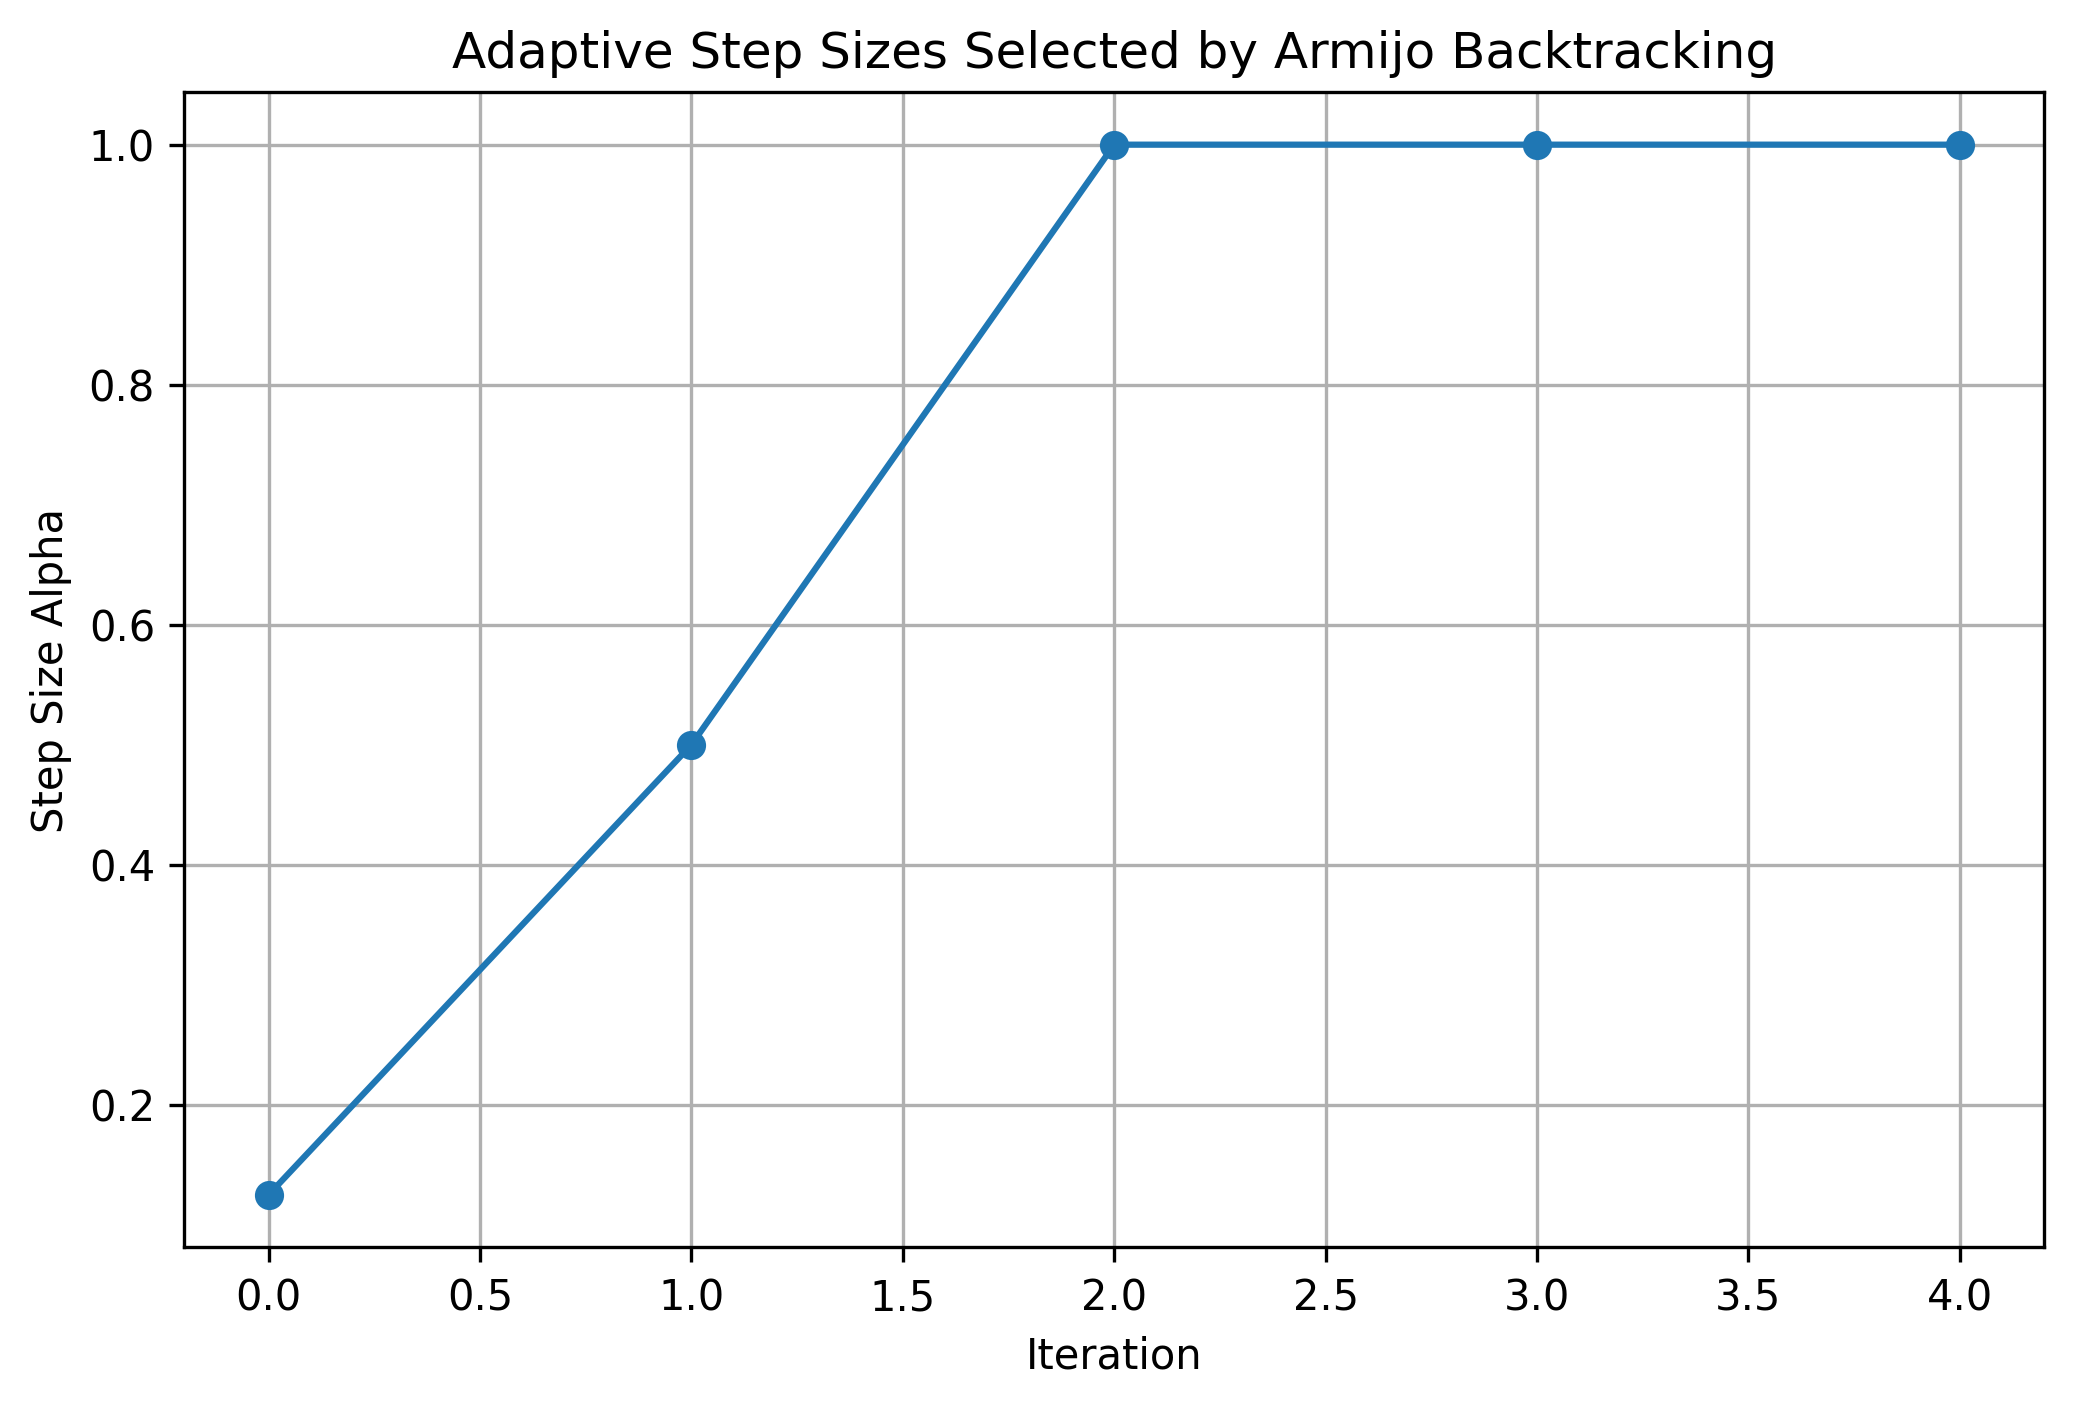
\includegraphics[width=0.75\textwidth]{figures/armijo_alpha_history.png}
\caption{Adaptive step sizes selected by Armijo backtracking}
\label{fig:armijo_alpha_history}
\end{figure}

The step-size plot shows the adaptive character of the method clearly. In the first iteration, the algorithm selects a small value of
\[
\alpha_k.
\]
This prevents the method from taking an unstable full Newton step. In the later iterations, the selected step size increases. Once the iterates are close enough to the root, the method accepts
\[
\alpha_k=1,
\]
which corresponds to the full Newton step.

Table~\ref{tab:armijo_comparison} summarizes the numerical results.

\begin{table}[h!]
\centering
\caption{Comparison of Newton-type methods with Armijo stabilization}
\label{tab:armijo_comparison}
\begin{tabular}{|c|c|c|c|}
\hline
Method & Iterations & Final Residual & Converged \\ \hline
Newton & 75 & \(4.45\times10^{40}\) & No \\ \hline
Constant Damped Newton & 58 & \(1.15\times10^{-7}\) & Yes \\ \hline
Adaptive Armijo Newton & 5 & \(3.06\times10^{-9}\) & Yes \\ \hline
\end{tabular}
\end{table}

The comparison shows the advantage of adaptive damping. Classical Newton's method is fast only when the full step is reliable. Constant damping improves stability, but it uses the same step size at every iteration and therefore converges slowly. The Armijo-based method adjusts the step size according to the behavior of the merit function. For this reason, it can avoid unstable steps at the beginning and still recover the fast local behavior of Newton's method near the solution.

This experiment supports the main idea of this chapter: optimization-based line-search methods are not only theoretical tools, but they can also improve the practical behavior of nonlinear equation solvers.

\section{Discussion}

The experiments presented in this chapter demonstrate that the practical behavior of Newton-type methods depends strongly on step-size control and stabilization strategies.

Classical Newton's method is known for its very rapid local convergence. When the initial approximation is sufficiently close to the root and the Newton direction is reliable, the method usually converges within only a few iterations. However, the numerical experiments showed that the method may also become highly unstable when these conditions are not satisfied. In the selected test problem, the full Newton step produced excessively large updates and caused divergence.

The constant damped Newton method improved stability by restricting the step size. The smaller updates prevented the divergence observed in the classical Newton iteration. Nevertheless, the use of a fixed damping parameter also introduced an important disadvantage. Since the same step size was used throughout the entire iteration process, the method converged much more slowly, even after the iterates entered a stable region near the root.

The adaptive Armijo-based method provided a more balanced behavior. Instead of relying on a fixed damping parameter, the algorithm adjusted the step size according to the local behavior of the merit function. During unstable stages of the iteration, the method selected smaller step sizes in order to maintain sufficient decrease of the residual. Once the iterates approached the solution, the algorithm accepted larger step sizes and recovered the fast convergence behavior of Newton's method.

These observations highlight one of the central ideas connecting optimization and nonlinear equation solving. In both areas, the quality of the search direction alone is often insufficient. Controlling the length of the iteration step is equally important for obtaining stable and efficient numerical behavior.

The experiments also demonstrate that optimization-inspired techniques such as merit functions, line-search procedures, and Armijo conditions can significantly improve the robustness of nonlinear solvers. Although these ideas originate mainly from optimization theory, they naturally extend to root-finding problems because both approaches depend heavily on iterative reduction of residuals.

Overall, the adaptive damped Newton method illustrates how optimization-based stabilization strategies can improve nonlinear equation solving without completely sacrificing the rapid local convergence properties of Newton's method.
\chapter{\MakeUppercase{Conclusion}}

\section{Summary of Findings}

In this thesis, several numerical methods for solving nonlinear equations and systems of nonlinear equations were studied from both theoretical and computational perspectives.

For single nonlinear equations, the bisection, secant, Newton, damped Newton, and Brent methods were examined. Their mathematical foundations, convergence behaviors, advantages, limitations, and possible failure cases were discussed in detail. In addition, illustrative examples were presented in order to demonstrate how the methods behave during the iterative process.

For nonlinear systems, multivariable Newton and Broyden methods were investigated. The role of the Jacobian matrix, convergence properties of Newton-type methods, and quasi-Newton approximations were analyzed both theoretically and numerically.

All methods considered in this thesis were implemented in Python using a consistent computational structure. Numerical experiments were performed in order to compare the methods in terms of convergence speed, residual reduction, robustness, and stability. The experiments showed that the theoretical convergence properties of the methods are clearly reflected in their computational behavior.

The study also investigated the relationship between nonlinear equation solving and optimization. In particular, residual minimization, damping strategies, line-search techniques, and the Armijo condition were discussed from an optimization perspective. An adaptive damped Newton method based on Armijo backtracking was implemented and compared with the classical Newton method and the constant damped Newton method. The numerical results demonstrated that adaptive damping can improve stability and convergence behavior, especially for difficult initial approximations.

Overall, the study showed that nonlinear equation solving is not only a theoretical mathematical topic but also an important component of scientific computing, optimization, and numerical simulation.

\section{Limitations}

The scope of this thesis was intentionally restricted to relatively small and medium-sized nonlinear problems. Large-scale sparse systems, high-dimensional optimization problems, and advanced large-scale numerical solvers were not considered in detail.

In addition, the numerical experiments mainly focused on convergence behavior, residual reduction, and stability properties. Computational performance measures such as execution time, memory usage, and scalability were not investigated extensively.

Another limitation is that only a selected group of classical and Newton-type methods was considered. More advanced techniques such as Levenberg--Marquardt methods, adaptive trust-region algorithms, and higher-order quasi-Newton approaches were outside the scope of this study.

Finally, the implementations were developed primarily for educational and experimental purposes. Although the algorithms were tested carefully, the software was not designed as a fully optimized numerical library.

\section{Future Work}

Several possible extensions of this work may be considered in future studies.

One possible direction is the investigation of large-scale nonlinear systems arising in scientific computing, engineering, and applied mathematics. In such problems, sparse matrix techniques, iterative linear algebra solvers, and efficient Jacobian approximations become increasingly important.

Another possible extension is the study of more advanced optimization-based nonlinear solvers. In particular, adaptive line-search strategies, trust-region methods, and modern quasi-Newton techniques may provide improved robustness and efficiency.

The implementations developed in this thesis may also be extended into a more comprehensive numerical software package containing visualization tools, benchmarking utilities, automated testing systems, and interactive experiment environments.

Finally, the relationship between nonlinear equation solving, optimization, and machine learning presents another interesting research direction. Many modern machine learning algorithms rely heavily on optimization techniques, and Newton-type approaches continue to play an important role in large-scale computational problems.

\bibliographystyle{apalike}
\bibliography{bibliography/references}

\end{document}